\documentclass[a4paper, 12pt]{article}

% Import the settings.sty file for the preamble
\usepackage{settings}
% Import necessary packages
\usepackage{amsmath} % for mathematical symbols and equations
\usepackage{amssymb} % for additional mathematical symbols
\usepackage{amsfonts} % for mathematical fonts
\usepackage{mathtools} % for additional mathematical symbols
\usepackage{bm} % for bold math symbols
\usepackage{amsthm} % for theorem environments
\usepackage{graphicx} % for including graphics
\usepackage{hyperref} % for hyperlinks
\usepackage{changepage} % for adjusting margins
\usepackage{subcaption} % for subfigures

\addbibresource{zotero-library.bib} % specify the bibliography file

% Set up the template for the technical report
\title{STAT9700 Final Project: Conformal Prediction}
\author{Joseph Rudoler}
\date{\today}

\newtheorem{theorem}{Theorem}
\newtheorem{lemma}{Lemma}

\begin{document}

\maketitle

\abstract{
    \footnotesize
    Conformal prediction is a model-agnostic framework for constructing valid prediction sets (and corresponding hypothesis tests) without making any assumptions about the underlying data
    distribution.
    As modern machine learning systems continue to scale in both size and complexity,
    the ability to make valid predictions without making assumptions about the training data or model is becoming increasingly important. In particular, the success and ubiquity
    of deep and over-parameterized neural networks has led to a growing interest in
    techniques that can provide statistically rigorous uncertainty quantification for models that are effectively a ``black box''.
    In this report, we will provide an overview of the conformal inference framework and some important results, discuss some extensions and demonstrate an application of conformal inference in a natural language processing setting.
}

\section*{Introduction}
Conformal prediction (also known as conformal inference) was first introduced by \textcite{vovkMachineLearningApplicationsAlgorithmic1999} and has seen a surge of interest within the last decade. Contributing to this increased interest is the growing popularity of machine learning models which are effectively ``black boxes'' - that is, models which have so many parameters and such flexible architectures that it is nearly impossible do inference on their learned parameters. Deep neural networks with millions or billions of parameters are now ubiquitous in important tasks in computer vision, natural language processing, and reinforcement learning. These models are for safety-critical applications like medical diagnosis or autonomous driving, making uncertainty quantification paramount for their deployment.

Conformal prediction provides a framework for constructing prediction sets (in continuous settings like regression, prediction intervals) with rigorous coverage guarantees for \textit{any} model at test time. The only assumption required is that the data are exchangeable, and we will see examples later of how this assumption can be relaxed.

This report is organized as follows: We will begin with an overview of the conformal prediction framework and some important results, then briefly summarize some key extensions, and finally provide an example application of conformal prediction to text classification with a large language model.

\section{Foundations}
This section will begin with a discussion of some conformal prediction basics,
loosely following~\cite{angelopoulosGentleIntroductionConformal2022}.
This will include an abbreviated proof of the validity of conformal prediction sets for exchangeable data,
and an overview of some important applications and extensions of conformal prediction.
We will then discuss how conformal prediction can be used in a cross-validation setting to obtain confidence intervals with rigorous coverage guarantees \autocite{barberPredictiveInferenceJackknife2020}.
Next, we will discuss in more detail how conformal prediction can be married to kernel density estimation to obtain prediction sets with asymptotic efficiency
guarantees \autocite{leiDistributionFreePrediction2013}.
Finally, we will see what happens when we try to apply conformal prediction to
non-exchangeable data \autocite{barberConformalPredictionExchangeability2023}.

\subsection*{Conformal prediction basics}
The central goal of conformal prediction is to construct prediction sets which have coverage guarantees at
a specified confidence level $1-\alpha$. That is, given the task of mapping some inputs
$X \in \mathcal{X} \mapsto \mathcal{Y}$, we ideally want to construct a set $C(X) \subset \mathcal{Y}$ such that
$\P(Y \in C(X)) \geq 1 - \alpha$ for all $X \in \mathcal{X}$. As it turns out,
when the data are i.i.d. or exchangeable, this is pretty easy. The definition of conformal prediction sets and the formal statement of the coverage
guarantee, for exchangeable data, is as follows:
\begin{theorem}[Conformal prediction sets for exchangeable data]
    Suppose that $(X_i, Y_i)$ for $i = 1, \ldots, n$ and $(X_{\text{test}}, Y_{\text{test}})$ are exchangeable random variables. \\
    Define
    \[
        \hat{q} = \inf \left\{ q: \frac{\left| i : s(X_i, Y_i) \leq q \right|}{n} \geq \frac{\lceil (n+1)(1-\alpha) \rceil }{n} \right\}
    \]
    where $\lceil \cdot \rceil$ is the ceiling function.\\
    Define a prediction set
    \[
        C(X) = \left\{ y: s(X, y) \leq \hat{q} \right\}
    \]
    Then \[ \P (Y_{\text{test}} \in C(X_{\text{test}})) \geq 1 - \alpha \]
    \label{thm:exchangeable_conformal_prediction}
\end{theorem}
Informally, we define a \textit{conformal score} function $s : (\mathcal{X}, \mathcal{Y} \mapsto \R) $ which
serves as a heuristic measure of how unlikely a given observation is (usually based on a trained model).
Then, for a test observation $X_{\text{test}}$ we predict the set of all $Y$ which are below approximately the $(1-\alpha)$ quantile of these scores on a calibration dataset.
This means that we're choosing a prediction set which contains all $Y$ which are ``not too unlikely'' given the calibration data.
Note that the coverage guarantee holds for any $s$, but the choice of $s$ will affect the size (and consequently, the usefulness) of the prediction set $C(X)$ - intuitively,
the less informative $s$ is, the larger $C(X)$ will need to be to achieve the desired coverage. \\
The proof of this coverage guarantee (with the simplifying assumption that $s(X_i, Y_i)$ are unique, to avoid handling ties) is as follows:
\begin{proof}
    Begin with a set of exchangeable pairs $(X_1, Y_1), \ldots, (X_n, Y_n), (X_\text{test}, Y_\text{test})$. We
    want to obtain a prediction set for $X_{\text{test}}$ which contains the true value $Y_\text{test}$ with probability at least $1-\alpha$.
    Assume without loss of generality that we have a model (e.g. a trained neural network) which can be
    used to compute a score $s(X, Y)$ for any $(X, Y)$ pair. \\
    % If the score function reflects how unlikely a pairing is according to the model, then the distribution of
    % scores on our calibration dataset reflects how unlikely our model thinks true labels are over this data distribution.
    We can sort the scores $s(X_i, Y_i)$ for $i = 1, \ldots, n$ in ascending order, and denote the $i$th smallest score by $s_{(i)}$.
    We set the threshold
    \[\hat{q} = \inf \left\{ q: \frac{\left| i : s(X_i, Y_i) \leq q \right|}{n} \geq \frac{\lceil (n+1)(1-\alpha) \rceil }{n}\right\}\]
    Since the scores are sorted (with no ties), we can see that $$\hat{q} = \begin{cases}
            s_{(\lceil (n+1)(1-\alpha) \rceil)} & \text{if } \alpha \geq \frac{1}{n+1} \\
            +\infty                             & \text{otherwise }
        \end{cases}$$
    And accordingly construct a prediction set:
    \[C(X) = \left\{ y: s(X, y) \leq \hat{q} \right\}\]
    What is the probability that $Y_{\text{test}} \in C(X_{\text{test}})$? This
    is where the exchangeability assumption is crucial. Since the data are exchangeable,
    $s_{\text{test}}$ is distributed identically to $s_{i}$ for any $i = 1, \ldots, n$.
    It follows that $s_{\text{test}}$ is equally likely to be fall into any of the $n+1$ intervals between the $n$ calibration scores.
    Formally, for any integer $k$ we have:
    \[ \P(s_{\text{test}} \leq s_{(k)}) = \frac{k}{n+1} \]
    In particular, we have:
    \[ \P(s_{\text{test}} \leq s_{(\lceil (n+1)(1-\alpha) \rceil)}) = \frac{\lceil (n+1)(1-\alpha) \rceil}{n+1} \geq 1 - \alpha \]
    Which proves the coverage guarantee.
\end{proof}

Part of the ``magic'' of conformal prediction is that this procedure can be applied
post-training to any model, for basically any prediction task. That means we can treat any
model as a ``black box'' and still obtain valid prediction sets without making any assumptions
about how the model was parameterized. While we assume that the data are exchangeable (i.e. identically distributed),
they need not be independent or to follow any particular distribution. We will see later
how this assumption can be relaxed to allow for non-exchangeable data. \\
To help solidify our intuition for conformal prediction, we include a simple outline of the conformal
procedure as described in \autocite{angelopoulosGentleIntroductionConformal2022} and concurrently expand the example case of
multi-label image classification:
\begin{enumerate}
    \item Given a pre-trained model, we \textbf{identify a heuristic notion of uncertainty} for the model's predictions. In image classification, we might use the softmax probabilities $\hat{f}(X)$ output by the a neural network.
    \item \textbf{Define a conformal score function $\bm{s(\cdot)}$} based on this uncertainty measure. For our example, we might define $s(X, Y)=1-\hat{f}(X)_Y$. This score function is lower for more likely image labels, and higher for less likely image labels.
    \item \textbf{Set a threshold} $\bm{\hat{q}}$ at the $ \frac{\lceil (n+1)(1-\alpha) \rceil }{n}$ quantile of the scores $s(X_i, Y_i)$ for $i = 1, \ldots, n$.
    \item \textbf{Construct a prediction set} $C(X_{\text{test}}) = \left\{ y: s(X_{\text{test}}, y) \leq \hat{q} \right\}$.
          In image classification, this is the set of all image labels with a score below the $\hat{q}$ quantile of scores on the calibration dataset. In other words,
          you add the mostly likely labels to the prediction set until their total probability mass under the distribution of scores on the calibration dataset is at least $1-\alpha$. Then
          the prediction set contains the true image label with probability at least $1-\alpha$.
\end{enumerate}
Again, we emphasize that the key to making conformal prediction sets \textit{useful}
lies in the choice of the score function $s$. While any $s$ provides sets which are valid
(in the sense that they have the desired coverage), a good choice of $s$ will result in a small prediction sets
which are also \textit{adaptive}. That is, the size of the prediction set will depend on how much uncertainty
the model has about the prediction.

\paragraph*{Split vs Full conformal prediction} In the above discussion, we assumed that we had access to a calibration dataset of exchangeable pairs $(X_i, Y_i)$ for $i = 1, \ldots, n$ which is non-overlapping with the training data used to fit the model. This is known as \textit{split conformal prediction} (or \textit{inductive conformal prediction}), and it has the desirable property of allowing a user to evaluate a pre-trained model without doing any additional training. However, in some cases we may not have enough data to split into training and calibration sets. In this case, we can use the full dataset to construct a valid prediction set. This is known as \textit{full conformal prediction} (or \textit{transductive conformal prediction}). Full conformal prediction is computationally more expensive than split conformal prediction, as it involves fitting a new model for each possible value $y \in \mathcal{Y}$ and recomputing the scores. However, it is still possible to obtain valid prediction sets without splitting the data. In full conformal prediction, we construct an augmented dataset of exchangeable pairs $(X_i, Y_i)$ for $i = 1, \ldots, n$ by adding a new observation $(X_{n+1}, y)$ to the training data.
We then fit a model to this augmented dataset and compute the scores $s^y(X_i, Y_i)$ for $i = 1, \ldots, n+1$.
The threshold $\hat{q}$ is now dependent on the value $y$ we added to the training data:
\[ \hat{q}^y = \inf \left\{ q: \frac{\left| i : s^y(X_i, Y_i) \leq q \right|}{n} \geq \frac{\lceil (n+1)(1-\alpha) \rceil }{n} \right\} \]
And the prediction set becomes:
\[ C(X) = \left\{ y: s^y(X_{n+1}, y) \leq \hat{q}^y \right\} \]
Intuitively, this is testing if the the new observation $(X_{n+1}, y)$ is exchangeable with all of the other observations, under the null hypothesis that $y$ is the true label for $X_{n+1}$.
The next section discusses a connection between full conformal prediction and kernel density estimation which allows us to obtain prediction sets with asymptotic efficiency guarantees.

\subsection*{Holdout methods: Jackknife+ and CV+}
To avoid overfitting, it is common to train a model on a partial dataset and reserve the remaining observation as a holdout for validation (or test). Split conformal prediction, as described above, is an example of a method with a single holdout - the conformal procedure is calibrated on part of the data and then applied to the remaining holdout data. (Actually, in practice there is a third set of data - the training data - which is used to fit the model, but not used in the conformal procedure.)

\textcite{barberPredictiveInferenceJackknife2020} discuss the application of conformal prediction to iterative holdout methods, which are a popular approach to uncertainty quantification in machine learning.\\

Before proceeding, we define some added notation. Take $\hat{q}^+\{\cdot \}$ is the $\frac{\lceil (n+1)(1-\alpha) \rceil }{n}$ quantile, and $\hat{q}^-\{\cdot \}$ is the $\frac{\lfloor (n+1)\alpha \rfloor }{n}$ quantile. We will also use the notation $\hat{f}_{-i}(X_i)$ to denote the model fit to the full dataset without the $i$th observation.

The original jackknife method involves fitting a model to the full dataset, and then generating an empirical distribution of test residuals obtained by computing the for each observation from a model fit to the full dataset without that observation. We can use the quantiles of this distribution to construct a confidence region. Specifically, we can define a prediction set for a new observation $X_{n+1}$ as:
\[ \hat{C}^{JK}(X_{n+1}) = \hat{f}(X_{n+1}) \pm \hat{q}\{ |Y_i - \hat{f}_{-i}(X_i)|\} \]
Or, equivalenty:
\[ \hat{C}^{JK}(X_{n+1}) = \left[ \hat{q}^{-}\left\{ \hat{f}(X_{n+1}) - |Y_i - \hat{f}_{-i}(X_i)|\right\}, \hat{q}^{+}\left\{ \hat{f}(X_{n+1}) + |Y_i - \hat{f}_{-i}(X_i)|\right\} \right] \]
While this procedure has been shown to provide good empirical coverage, it is not valid in general - only in the case where the model meets certain stability criteria \autocite{steinbergerConditionalPredictiveInference2022}.

\textcite{barberPredictiveInferenceJackknife2020} propose a conformalized version of the jackknife method, which they call Jackknife+. In particular, they define the prediction set for a new observation $X_{n+1}$ as:
\[ \hat{C}^{JK+}(X_{n+1}) = \left[ \hat{q}^{-}\left\{ \hat{f}_{-i}(X_{n+1}) - |Y_i - \hat{f}_{-i}(X_i)|\right\}, \hat{q}^{+}\left\{ \hat{f}_{-i}(X_{n+1}) + |Y_i - \hat{f}_{-i}(X_i)|\right\} \right] \]

The key difference here is that the test point for $X_{n+1}$ is variable, since it is produced by the iterative model fits excluding observation $i$. So, instead of getting a symmetric interval around $\hat{f}(X_{n+1})$, we get an interval about the median of $\{\hat{f}_{-i}(X_{n+1})\}$ which is not symmetric in general.

\subsection*{Density estimation}
Generating conformalized prediction sets can be cast as a problem of estimating
density level sets for an unknown probability distribution \autocite{leiDistributionFreePrediction2013}.
Consider a sequence of i.i.d. data drawn from some unknown distribution with density $p(y)$.
If we want to find a set $C$ for a new observation such that
$\P(Y \in C) \geq 1 - \alpha$, this is equivalent to finding an estimated density level set
$$L(t_\alpha)=C_\alpha=\{y: \hat{p}(y) \geq t_\alpha\} \quad \text{where} \quad t_\alpha = \inf \{t: \P(Y \in L(t)) \geq 1 - \alpha\}$$
We will deal with this more general notation in this section (following the original paper), but it is worth noting that in typical machine learning applications we deal with a model that predicts $Y$ based on some features $X$. The goal is then using that model's predictions to find a set $C(X)$ such that the probability $\P(Y \in C(X) ) \geq 1 - \alpha$.\\
Note that if $\hat{p}(y)$ were estimated perfectly, we would have no need to conformalize the density level set --
we would simply greedily add the most likely observations to the set until we reached the desired coverage.
However, in practice we will need to estimate $\hat{p}(y)$ from a finite sample
of data and inevitably introduce some error which might cause us to undercover or overcover. \\
We now consider the standard kernel density estimator (KDE) with kernel fuction $K$ and bandwidth $h$, \\
\[\hat{p}(u) = \frac{1}{n} \sum_{i=1}^n K_h(u-Y_i) \]
For our score function, we will use an augmented version of the KDE which is estimated on the augmented dataset $Y_1, \ldots, Y_{n+1}$ where $Y_{n+1}= y$:
\[ \hat{p}^y(u) = \frac{1}{n+1} \sum_{i=1}^{n+1} K_h(u-Y_i) \]
The paper defines a conformal score a bit differently than we have so far, such that higher conformal scores correspond to more likely labels. This is helpful in order to more naturally frame the prediction set as a density level set. So we have $s^y(y) = \hat{p}^y(y)$, and we set the threshold $\hat{q}^y$ at the $ \frac{\lfloor (n+1)\alpha \rfloor }{n}$ quantile of the scores $s^y(X_i, Y_i)$ for $i = 1, \ldots, n$ and take the valid prediction set to be:
\[ \hat{C}_\alpha = L(\hat{t}_\alpha) = \left\{ y: s^y(y) \geq \hat{q}^y \right\} \]
So, our prediction set is all $y$ such that the estimated density level set $L(\hat{t}_\alpha)$ contains $y$ with probability at least $1-\alpha$. (Note that this is equivalent to making the score function $s^y(y)=-\hat{p}^y(y)$, defining $\hat{q}^y$ at the $ \frac{\lceil (n+1)(1-\alpha) \rceil }{n}$ quantile of the scores, taking a prediction set $\hat{C}_\alpha = \left\{ y : s^y(y)\leq \hat{q}^y \right\}$.)  \\
Since this kernel density estimator is expensive to compute for every possible value of $y$, \citeauthor{leiDistributionFreePrediction2013} propose a faster approximation that sandwiches the kernel density estimator between two simpler estimators ($L^-$ and $L^+$) and preserves finite-sample validity. That is, they they define the following lemma:
\begin{lemma}
    Let $\hat{C}_\alpha$ be the conformal prediction set based on the KDE with kernel function $K$, and assume $\sup_u |K(u)|=K(0)$. Let $Y_{(1)} \ldots Y_{(n)}$ be the data in increasing order by their estimated kernel density.
    \[L^-= L\left(\hat{p}(Y_{(\lfloor (n+1)\alpha \rfloor)})\right) \quad \text{and} \quad
        L^+= L\left(\hat{p}(Y_{(\lfloor (n+1)\alpha \rfloor)})\right) - \frac{1}{nh} \sup_{u, u'} |K(u) - K(u')| \]
    Then
    \[ L^- \subseteq \hat{C}_\alpha \subseteq L^+ \]
\end{lemma}

Importantly, this sandwiching technique also provides lower and upper bounds on the efficiency of the kernel density estimator, which itself is harder to analyze. \textcite{leiDistributionFreePrediction2013} proceed to show that this procedure is asymptotically efficient at rate $r_n=(\frac{\log n}{n})^{c_{p_\alpha}}$ where $c_{p_\alpha}$ is a constant depending on the smoothness of the true underlying density. By efficient, we mean that probability of the loss $R(\hat{C}_\alpha, C_\alpha) = \mu(\hat{C}_\alpha \setminus C_\alpha) \leq \mu(\hat{C}_\alpha) - \mu(C_\alpha)$ exceeding $r_n$ converges to zero as $n \to \infty$.

It is worth noting as well that while the asymptotic efficiency of the kernel density estimator is only proven for the full conformal prediction procedure, kernel density estimation can be used to obtain valid prediction sets in the split conformal prediction setting as well.

\paragraph*{Conformalized Bayes.} Before moving on to the next section, we will mention that framing conformal prediction as a density level set estimation problem also connects nicely to Bayesian inference. In particular, we can choose the conformal score function to be the posterior predictive density of the label given the data, and the prediction set will be the density level set with coverage guarantee $1-\alpha$. ``Conformalized Bayes'' allows us to obtain valid prediction sets for Bayesian models without making any assumptions about the correctness of the model or the data distribution - in this sense it mitigates concerns about misspecified priors. \textcite{hoffBayesoptimalPredictionFrequentist2021} shows that under certain conditions, this procedure is Bayes optimal (in the sense that it minimizes the Bayes risk among all valid prediction sets).

\subsection*{Beyond exchangeability}

\section{Extensions and related work}
In this section, we further discuss two crucial extensions of conformal inference
to settings with non-exchangeable data \autocite{gibbsAdaptiveConformalInference2021, tibshiraniConformalPredictionCovariate2020}.
We will also discuss some related work on uncertainty quantification for deep neural networks that lies outside the conformal inference framework

\subsection*{Learn then test}
See \autocite{angelopoulosLearnThenTest2022}. \\
Maybe go more specifically into conformal language modeling \autocite{quachConformalLanguageModeling2023}.

\section{Application: Adaptive Conformal Prediction for Text Classification}
In this section, we will provide a case study of how conformal prediction can be used to obtain
prediction sets with rigorous coverage guarantees for text classification with a large language model (LLM). We will
compare a naive conformal prediction procedure with an adaptive conformal prediction procedure, and show that the
adaptive score can lead to smaller prediction sets while preserving valid coverage.

\paragraph*{Model.} We classify text with the transformer-based language model BART \autocite{lewisBARTDenoisingSequencetoSequence2019},
finetuned on the Multi-Genre Natural Language Inference (MNLI) categorized text corpus \footnote{\url{https://huggingface.co/datasets/multi_nli}},
as proposed by \textcite{yinBenchmarkingZeroshotText2019} for zero-shot text classification. The approach is to treat the task of text classification as a natural language inference (NLI) task, where the premise is the text to be classified and the hypothesis is a statement about the label like ``This text is about politics''. The model computes the probability that the hypothesis is true given the premise, and we repeat this for each label independently.

We note that this model is no longer state of the art, but it is more lightweight (400 million parameters) than the larger and more performant models which have gained prominence (e.g. Meta's Llama2 models range from 7-70 billion parameters), and therefore more suitable for fast inference on a laptop.
Since we are interested in demonstrating the utility of conformal prediction, we do not need to use the most powerful model available.
We will see that this model results in prediction sets which are fairly large, and it is likely that a more powerful model would result give us better heuristic uncertainty estimates and therefore smaller prediction sets.


\paragraph*{Data.} Our prediction task is to classify text from a new data source, a Kaggle dataset of text documents belonging to 5 new categories\footnote{\url{https://www.kaggle.com/datasets/sunilthite/text-document-classification-dataset/data}}. These categories -- Politics, Sport, Technology, Entertainment, and Business -- are mostly nonoverlapping with the categories in the MNLI corpus. The one exception being Politics, which is similar to the Government genre in MNLI -- we will see that this category is, unsurprisingly, the easiest to classify. Of course, BART's original training data surely contained text related to all of these genres (which is why we expect it have enough knowledge to be capable of zero-shot classification), but it was not specifically trained to classify them. We split this Kaggle dataset, using half the data for calibration and the other half for testing.

\paragraph*{Code} All the code for this project is available at \url{https://github.com/jrudoler/rudoler-stat9700-conformal}. This includes the code for language model inference, conformal prediction, and the code used to generate the figures in this report. We use the HuggingFace implementation of \texttt{bart-large-mnli}\footnote{\url{https://huggingface.co/facebook/bart-large-mnli}}, and set up a zero-shot text classification pipeline with the \texttt{transformers} library \autocite{wolfHuggingFaceTransformersStateoftheart2019}.

\subsubsection*{Conformal scores}
We will compare two different choices of score function $s$ for the conformal prediction procedure:
\begin{enumerate}
    \item \textbf{Nonadaptive}: We just use the predicted probability of each label independently to compute the score. That is, for a given text document $X$, we compute the score \[s(X, y) = 1 - \hat{f}(X)_y \] for each label $y$.
    \item \textbf{Adaptive}: We consider the predicted probability of all labels simultaneously in computing the score. Specifically we reorder the labels by descending probability, such that $\hat{f}(X)_{(1)}$ is the most likely label, $\hat{f}(X)_{(2)}$ is the second most likely label, and so on. We define $k$ such that $\hat{f}(X)_{(k)} = y$, and compute the score: \[ s(X, y) = \sum_{j=1}^{k} \hat{f}(X)_{(j)} \] Basically, we add up the predicted probabilities of all the labels in descending order up to and including the true label, $y$.
\end{enumerate}

\textcite{angelopoulosUncertaintySetsImage2022} discuss adaptive prediction sets in detail in the context of image classification, and introduce the adaptive score function we use here.

\paragraph*{Results} We evaluate the prediction sets produced via conformal prediction with each of the two score functions described above. Figure \ref{fig:coverage} shows the overall coverage of the prediction sets for each score function, as well as the conditional coverage for each category. Figure \ref{fig:set_size} shows the average size of the prediction sets for each score function, again both overall and for each category.








% include vertically stacked subfigures for coverage
\begin{figure}[ht]
    \centering
    \begin{subfigure}[b]{0.8\linewidth}
        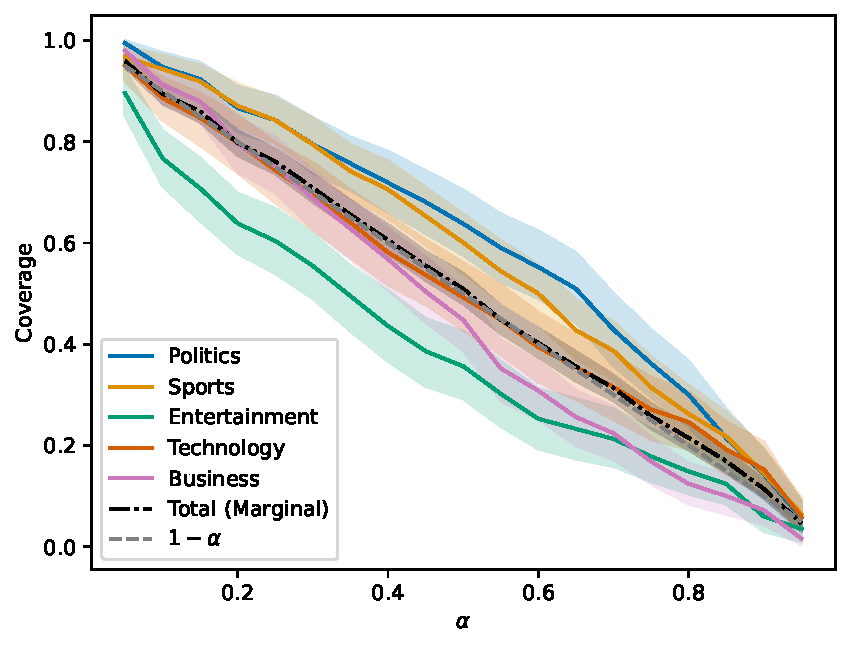
\includegraphics[width=\linewidth]{figures/nonadaptive_conditional_coverage.pdf}
        \caption{Nonadaptive conformal prediction}
        \label{fig:nonadaptive_coverage}
    \end{subfigure}
    \begin{subfigure}[b]{0.8\linewidth}
        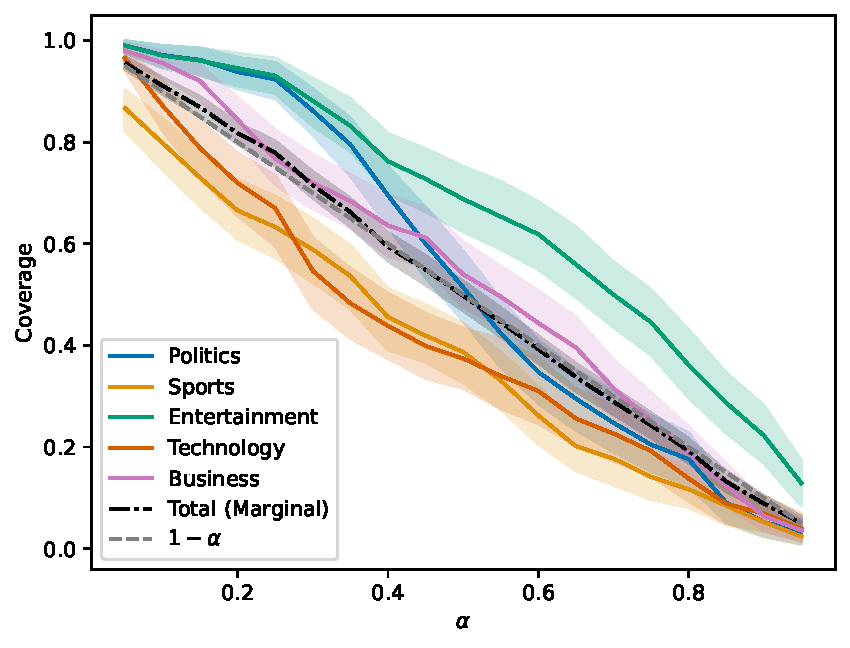
\includegraphics[width=\linewidth]{figures/adaptive_conditional_coverage.pdf}
        \caption{Adaptive conformal prediction}
        \label{fig:adaptive_coverage}
    \end{subfigure}
    \caption{Comparison of coverage for nonadaptive and adaptive conformal prediction for text classification. Both procedures have marginal coverage guarantees of $1-\alpha$. }
    \label{fig:coverage}
\end{figure}

% include vertically stacked subfigures for set size
\begin{figure}[ht]
    \centering
    \begin{subfigure}[b]{0.8\linewidth}
        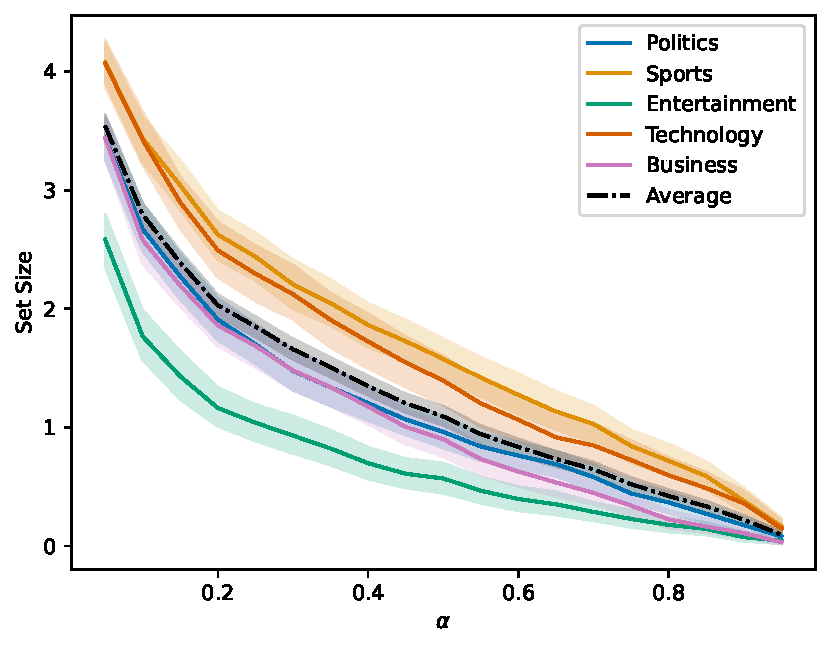
\includegraphics[width=\linewidth]{figures/nonadaptive_set_size.pdf}
        \caption{Nonadaptive conformal prediction}
        \label{fig:nonadaptive_set_size}
    \end{subfigure}
    \begin{subfigure}[b]{0.8\linewidth}
        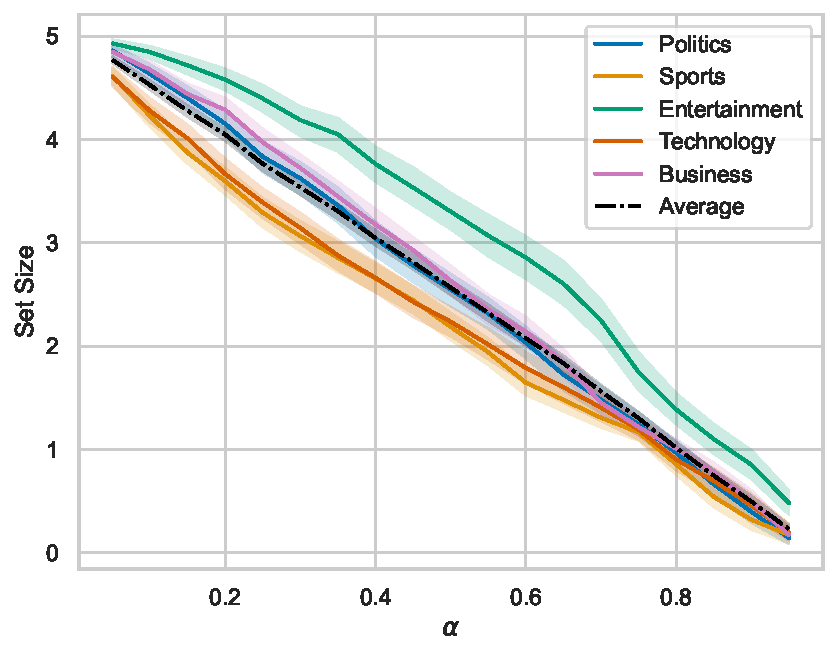
\includegraphics[width=\linewidth]{figures/adaptive_set_size.pdf}
        \caption{Adaptive conformal prediction}
        \label{fig:adaptive_set_size}
    \end{subfigure}
    \caption{Comparison of set size for nonadaptive and adaptive conformal prediction for text classification. The adaptive procedure improves coverage for the hardest categories by making their prediction sets larger.}
    \label{fig:set_size}
\end{figure}



\newpage
\printbibliography % print the bibliography

\end{document}
